\chapter{Aims}

% the code below specifies where the figures are stored
\ifpdf
    \graphicspath{{example_chapter/figures/PNG/}{example_chapter/figures/PDF/}{example_chapter/figures/}}
\else
    \graphicspath{{example_chapter/figures/EPS/}{example_chapter/figures/}}
\fi


% ----------------------------------------------------------------------
%: ----------------------- content ----------------------- 
% ----------------------------------------------------------------------

\section{Poop}
This is where I put one of my very own defined functions!

\begin{table}
\centering
\begin{tabular}{|c|ccc|r|}
	\hline
$k$ &  $x_1^k$    &   $x_2^k$  & $x_3^k$   & remarks  \\
	\hline
0   & -0.3 & 0.6 & 0.7  &  \\
1   & 0.47102965 & 0.04883157 & -0.53345964  & *\\
2   & 0.49988691 & 0.00228830 & -0.52246185 & $s_3$ \\
3   & 0.49999976 & 0.00005380 & -0.52365600  & \\
4   & 0.5 & 0.00000307 & -0.52359743  & $\epsilon < 10^{-5}$ \\
7   & 0.5 & 0 & -0.52359878  & $\epsilon < \xi $ \\
	\hline
\end{tabular}
\caption[A table of important values]{This is a table with {\emph very} important values!!!!!}
\label{important_values}
\end{table}
    
\uv plane
    $$ \pdfdx{f}{x} $$

\section{Blah} 
\lipsum
\begin{figure}
\centering
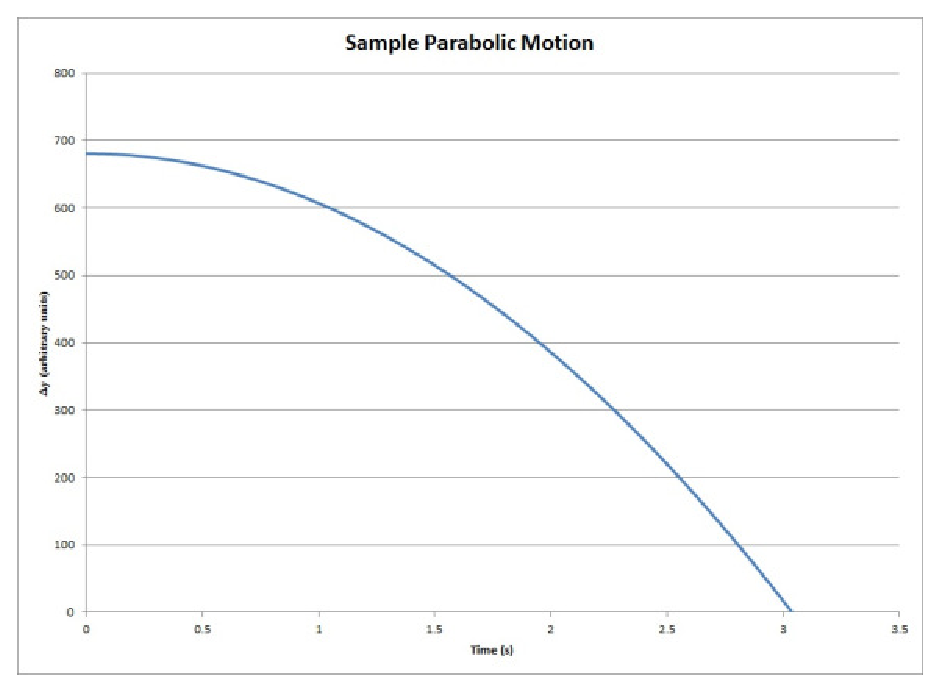
\includegraphics{parabolic_motion}
\caption[Parabolic Motion]{Here is parabolic motion as measured with science.}
\label{parabolic_motion}
\end{figure}
\lipsum
